\chapter{Turing Patterns}

\resp{Vladimir Ungureanu}

\section{Introduction}
Turing patterns arise in reaction–diffusion systems governed by coupled partial differential equations:
\begin{equation}
\frac{\partial u(x,t)}{\partial t}
= f(u,v) + D_{\text{act}} \,\nabla^{2} u(x,t)
\end{equation}
\begin{equation}
\frac{\partial v(x,t)}{\partial t}
= g(u,v) + D_{\text{inh}} \,\nabla^{2} v(x,t)
\end{equation}
where \(u\) is the activator density, \(v\) is the inhibitor density, \(f\) and \(g\) describe local dynamics, and \(D_{\text{act}}\) and \(D_{\text{inh}}\) are the diffusion constants.
In a discrete network, in place of the Laplacian operator we use the Laplacian matrix \(L_{ij} = A_{ij} - k_i\delta_{ij}\); thus the two equations become:
\begin{equation}
    \frac{d u_i(t)}{d t}
= f\bigl(u_i,\, v_i\bigr)
+ \varepsilon \sum_{j=1}^{N} L_{ij}\, u_j,
\label{eq:general_act}
\end{equation}
\begin{equation}
    \frac{d v_i(t)}{d t}
= g\bigl(u_i,\, v_i\bigr)
+ \sigma \varepsilon \sum_{j=1}^{N} L_{ij}\, v_j,
\label{eq:general_inh}
\end{equation}
where \(\varepsilon = D_{\text{act}}\) and \(\sigma = D_{\text{inh}}/D_{\text{act}}\). The roles of plane waves and wavenumbers are replaced by the eigenvectors \(\phi^{(\alpha)} = (\phi_1^{(\alpha)}, \ldots, \phi_N^{(\alpha)})\) and eigenvalues \(\Lambda_{\alpha}\) \((\alpha=1, \ldots, N)\) of the Laplacian matrix:
\begin{equation}
    \sum_{j=1}^N L_{ij}\phi_j^{(\alpha)} = \Lambda_\alpha\phi_i^{(\alpha)}.
\end{equation}
Performing a linear stability analysis of \eqref{eq:general_act} and \eqref{eq:general_inh}, the growth rate is
\begin{equation}
\lambda_{\alpha}
= \frac{1}{2}\left\{
  f_u + g_v + (1+\sigma)\,\varepsilon \Lambda_{\alpha}
  + \sqrt{\,4 f_v g_u + \bigl(f_u - g_v + (1-\sigma)\,\varepsilon \Lambda_{\alpha}\bigr)^2}
\right\}.
\end{equation}
From the condition that the critical growth rate \(\lambda_c\) touches the horizontal axis at its maximum, we find
\begin{equation}
\sigma_c
= \frac{\,f_u g_v - 2 f_v g_u
    + 2\sqrt{\,f_v g_u \,\bigl(f_v g_u - f_u g_v\bigr)}\,}{f_u^{2}}.
\end{equation}
The critical Laplacian eigenvalue(s) \(\Lambda_c\) for a given \(\varepsilon\) are
\begin{equation}
    \Lambda_c = \frac{(f_u - g_v)\sigma_c - \sqrt{|f_v|\,g_u\,\sigma_c}\,(\sigma_c + 1)}{\varepsilon \sigma_c(\sigma_c-1)}.
\end{equation}
The critical mode has component ratio \((1, B_c)\), where
\begin{equation}
    B_{c}
= \frac{-f_{u} + g_{v} + (\sigma_{c}-1)\,\varepsilon \Lambda_{c}
        + \sqrt{\,4 f_{v} g_{u} + \bigl(f_{u} - g_{v} - (\sigma_{c}-1)\,\varepsilon \Lambda_{c}\bigr)^{2}}}
       {2 f_{v}}.
\end{equation}

\begin{figure}[H] % or [htbp]
  \centering
  \begin{subfigure}{0.48\textwidth}
    \centering
    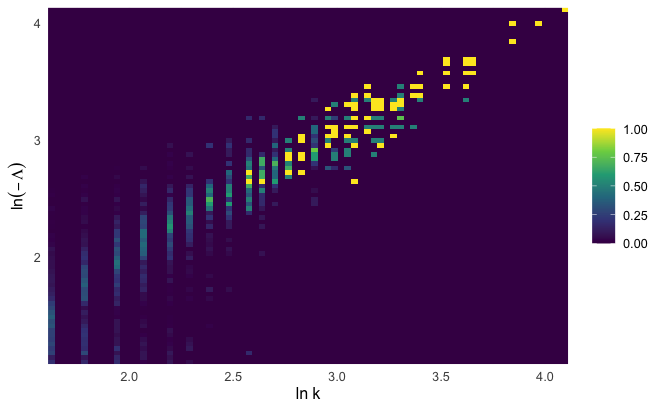
\includegraphics[width=\linewidth]{Graphs/heatmap_N=200.png}
    \caption{}
  \end{subfigure}\hfill
  \begin{subfigure}{0.48\textwidth}
    \centering
    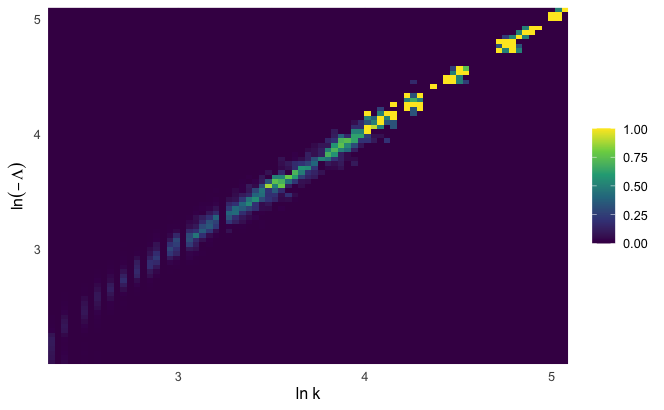
\includegraphics[width=\linewidth]{Graphs/heatmap_N=1000.png}
    \caption{}
  \end{subfigure}
  \caption{\textbf{Localization of Laplacian eigenvectors in scale-free networks.} The network sizes and mean degrees are \(N = 200\), \(\langle k\rangle = 10\) \textbf{(a)} and \(N=1000\), \(\langle k\rangle=20\) \textbf{(b)}. The density distribution of differentiated nodes within each subset of equal-degree nodes is shown for the entire set of Laplacian eigenvectors.}
  \label{fig:heatmap}
\end{figure}

Figure~\ref{fig:heatmap} shows that the differentiated nodes are approximately located along the diagonal axis, a fact that is model independent. Next, I study Turing pattern formation in scale-free networks for two different activator–inhibitor systems: the Mimura–Murray model and the Schnakenberg model.

\section{Mimura–Murray model}
The kinetics of the Mimura–Murray model are described by
\begin{equation}
    f(u,v) = \left( \frac{a + b\,u - u^{2}}{c} - v \right)u,
    \label{eq:Mimura_activator}
\end{equation}
\begin{equation}
g(u,v) = \bigl(u - 1 - d\,v\bigr)v,
\label{eq:Mimura_inhib}
\end{equation}
where \(a, b, c,\) and \(d\) are constants. In this study the parameters are \(a=35\), \(b=16\), \(c=9\), and \(d=2/5\), yielding the fixed point \((\bar{u}, \bar{v})\) with partial derivatives \(f_u=1.33\), \(f_v=-5\), \(g_u=10\), and \(g_v=-4\). Figure~\ref{fig:critical_find} shows the growth rate \(\lambda\) as a function of the eigenvalues \(\Lambda\). By locating where the curve touches zero, we find the critical eigenvalue(s) \(\Lambda_c\).

\begin{figure}[H] % or [htbp]
  \centering
  \begin{subfigure}{0.48\textwidth}
    \centering
    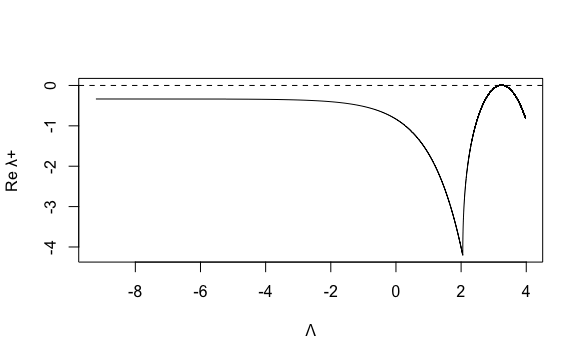
\includegraphics[width=\linewidth]{Graphs/growth-rate_vs_eigen189.png}
    \caption{\(\varepsilon=0.060\), \(\alpha_c=189\)}
  \end{subfigure}\hfill
  \begin{subfigure}{0.48\textwidth}
    \centering
    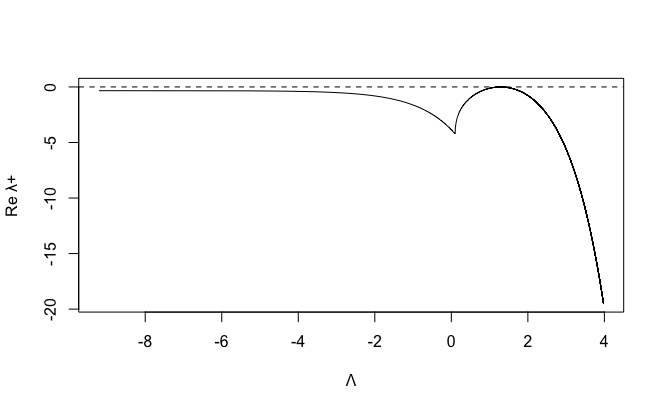
\includegraphics[width=\linewidth]{Graphs/growth-rate_vs_eigen15.png}
    \caption{\(\varepsilon=0.425\), \(\alpha_c=15\)}
  \end{subfigure}
  \caption{\textbf{Linear stability analysis.} Linear growth rates \(\lambda_\alpha\) of Laplacian modes \(\alpha=1,\ldots,N\)
  for the Mimura–Murray model on a scale-free network (\(N=200\) nodes and mean degree \(\langle k\rangle=10\)) are plotted as functions of the Laplacian eigenvalues \(\Lambda_\alpha\) for the critical ratio of diffusion constants \(\sigma=15.5\). The two curves correspond to \(\varepsilon=0.425\) and \(\varepsilon=0.060\).}
  \label{fig:critical_find}
\end{figure}

\begin{figure}[H] % or [htbp]
  \centering
  \begin{subfigure}{0.48\textwidth}
    \centering
    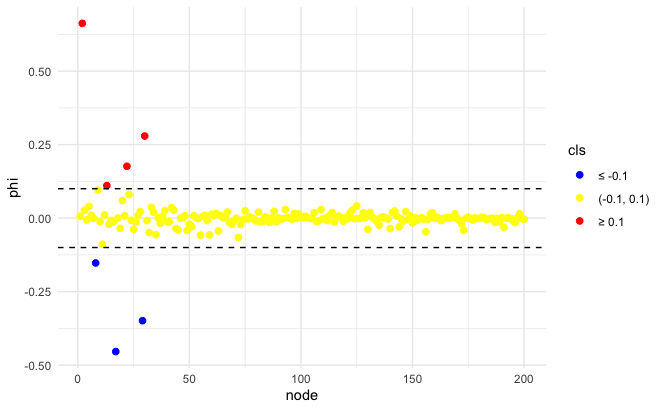
\includegraphics[width=\linewidth]{Graphs/phi189_vs_node_N=200.png}
    \caption{\(\alpha_c=189\)}
  \end{subfigure}\hfill
  \begin{subfigure}{0.48\textwidth}
    \centering
    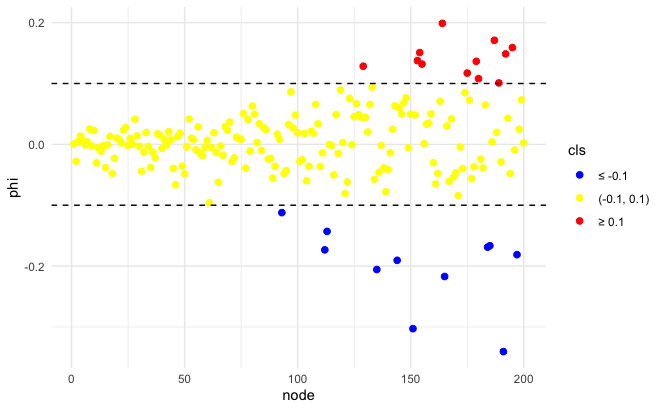
\includegraphics[width=\linewidth]{Graphs/phi15_vs_node_N=200.png}
    \caption{\(\alpha_c=15\)}
  \end{subfigure}

  \vspace{0.6em}

  \begin{subfigure}{0.38\textwidth}
    \centering
    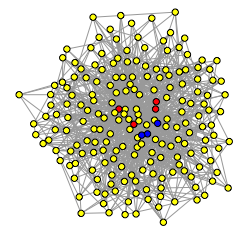
\includegraphics[width=\linewidth]{Graphs/phi189_network.png}
    \caption{\(\alpha_c=189\)}
  \end{subfigure}\hfill
  \begin{subfigure}{0.38\textwidth}
    \centering
    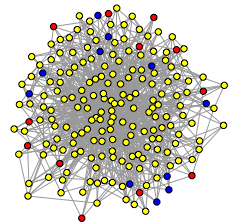
\includegraphics[width=\linewidth]{Graphs/phi15_network.png}
    \caption{\(\alpha_c=15\)}
  \end{subfigure}

  \caption{\textbf{Critical Turing modes of a scale-free network.} The network size is \(N=200\) and the mean degree is \(\langle k\rangle=10\). \textbf{a,b,} Critical eigenvectors \(\alpha_c=189\) \textbf{(a)} and \(\alpha_c=15\) \textbf{(b)} plotted against the node index \(i\). Node indices are sorted according to their degrees \(k_i\). \textbf{c,d,} The same critical eigenvectors \(\alpha_c=189\) \textbf{(c)} and \(\alpha_c=15\) \textbf{(d)}, displayed on the network.}
  \label{fig:critical_turing_modes1}
\end{figure}

In Figure~\ref{fig:critical_turing_modes1}, two critical Turing modes are displayed. Nodes are colored red when \(\phi_i^{(\alpha_c)} \ge 0.1\) (activator concentration significantly increased), blue when \(\phi_i^{(\alpha_c)} \le -0.1\) (significantly decreased), and yellow when \(-0.1 < \phi_i^{(\alpha_c)} < 0.1\). In the chosen representation, network nodes with larger degrees (hubs) are located in the center and the nodes with lower degrees in the periphery of the graph. Nodes with significant deviations of the activation level tend to have similar degrees.

\begin{figure}[H] % or [htbp]
  \centering
  \begin{subfigure}{0.48\textwidth}
    \centering
    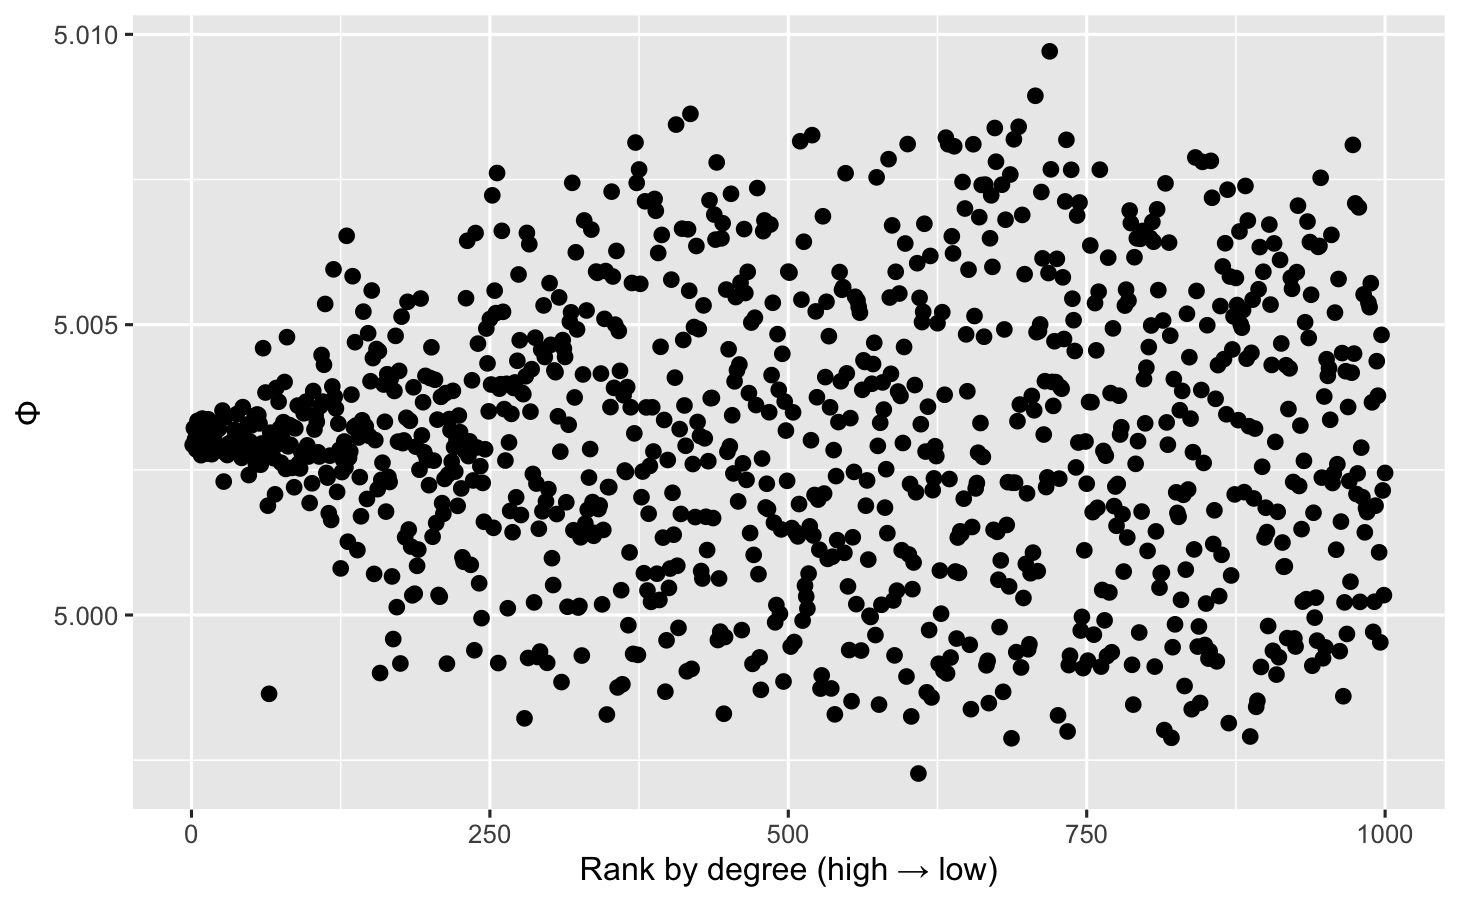
\includegraphics[width=\linewidth]{Graphs/Phi_vs_index.png}
    \caption{}
  \end{subfigure}\hfill
  \begin{subfigure}{0.48\textwidth}
    \centering
    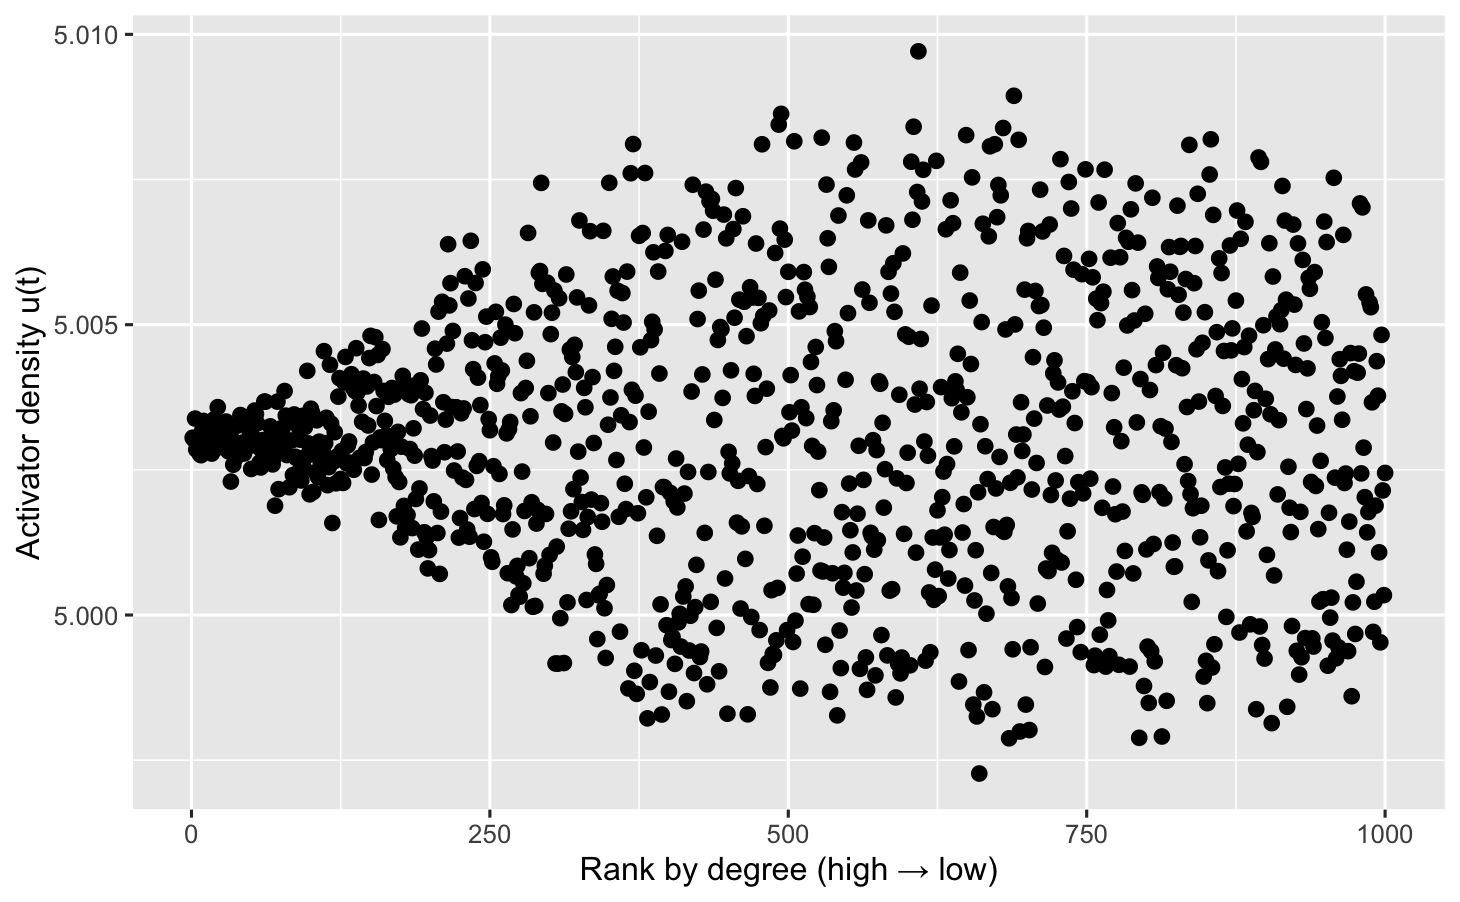
\includegraphics[width=\linewidth]{Graphs/Activator_density_vs_index_t = 200.png}
    \caption{}
  \end{subfigure}

  \vspace{0.6em}

  \begin{subfigure}{0.48\textwidth}
    \centering
    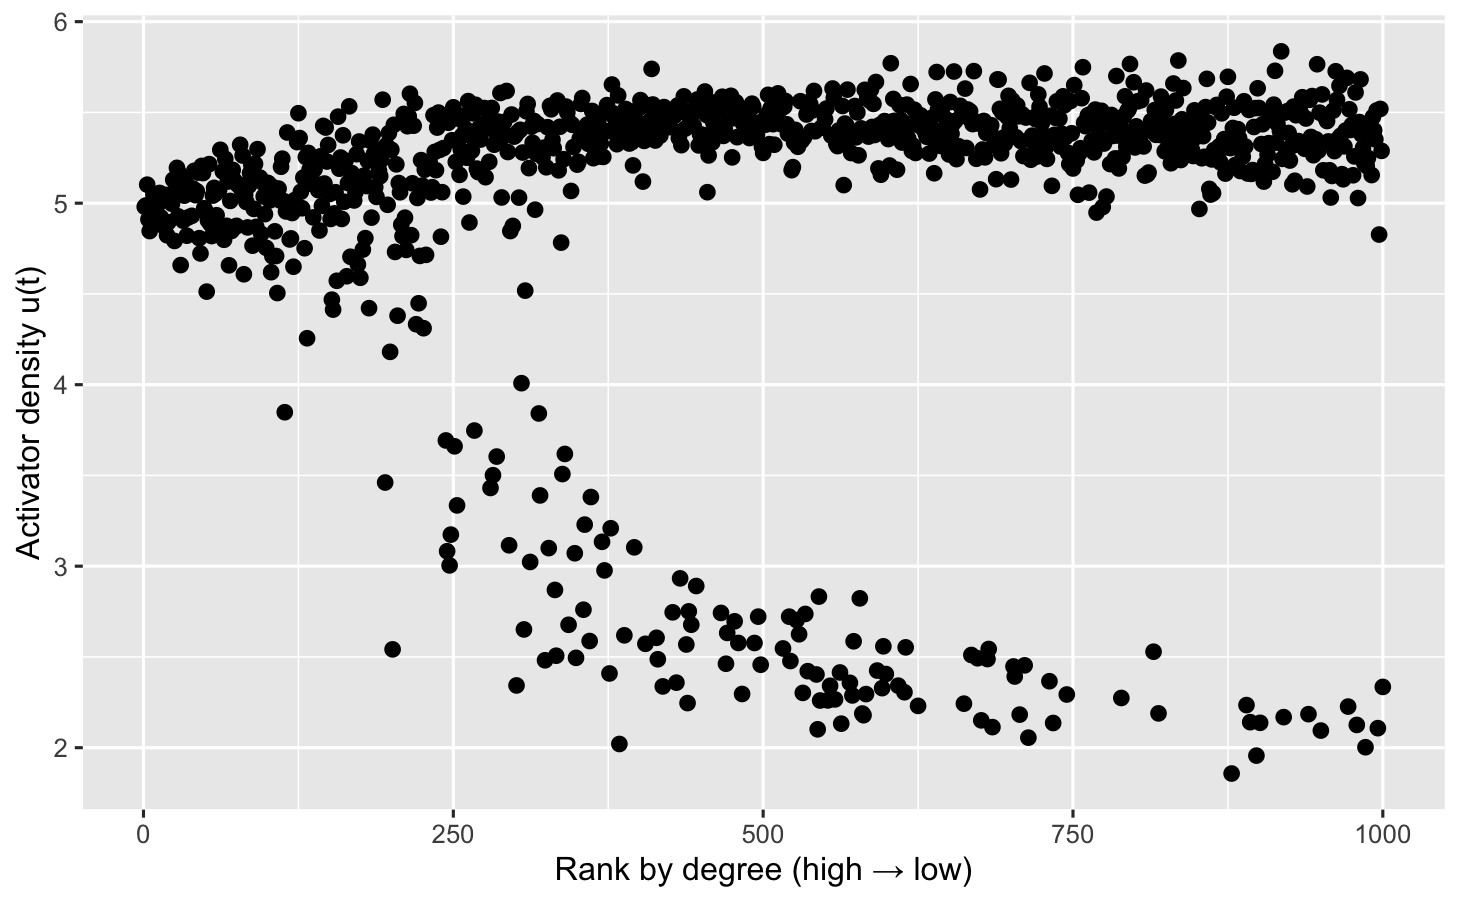
\includegraphics[width=\linewidth]{Graphs/Activator_denisty_vs_index_t=10000.png}
    \caption{}
  \end{subfigure}\hfill
 
  \caption{\textbf{Nonlinear evolution and a stationary Turing pattern.} The Mimura–Murray model with parameters \(\varepsilon=0.12\) and \(\sigma=15.6\) on a scale-free
network of size \(N=1{,}000\) and mean degree \(\langle k\rangle=20\). Nodes are ordered according to their degrees. \textbf{a,} The critical mode (the Laplacian eigenvector with
\(\alpha_c = 413\)). \textbf{b,} The activator pattern at the early evolution stage (\(t=200\)). \textbf{c,} The stationary activator pattern at the late stage (\(t=10{,}000\)).}
  \label{fig:mimura_evolution}
\end{figure}

Figure~\ref{fig:mimura_evolution} shows that at early stages the activator densities are similar to the critical eigenvector, but as time passes most nodes stabilize while some are kicked off the main group. The separation does not occur for nodes with high degrees. Up to this point, everything written is a reproduction of the results in the paper~\cite{paper}.

\section{Schnakenberg model}
The dynamics of the Schnakenberg model are described by
\begin{equation}
    f(u,v) = a - u + u^2 v,
\end{equation}
\begin{equation}
    g(u, v) = b - u^2 v,
\end{equation}
where \(a\) and \(b\) are constants~\cite{website}. In this study the parameters are \(a=0.2\) and \(b=1.3\), yielding the fixed point \((\bar{u}, \bar{v})\) with partial derivatives \(f_u=0.734\), \(f_v=2.25\), \(g_u=-1.734\), and \(g_v=-2.25\). In Figure~\ref{fig:sch_critical} it can be observed that, for this model, the critical eigenvectors tend to involve nodes with small degree. Also, for the critical eigenvector \(\phi^{(2)}\), the significantly deviated nodes appear polarized.

\begin{figure}[!htbp] % or [htbp]
  \centering
  \begin{subfigure}{0.43\textwidth}
    \centering
    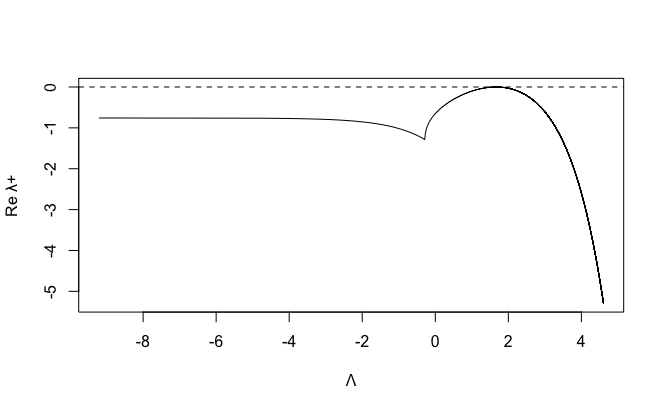
\includegraphics[width=\linewidth]{Graphs/Model2_growth-rate_vs_eigen66.png}
    \caption{\(\varepsilon=0.060\), \(\alpha_c=66\)}
  \end{subfigure}\hfill
  \begin{subfigure}{0.43\textwidth}
    \centering
    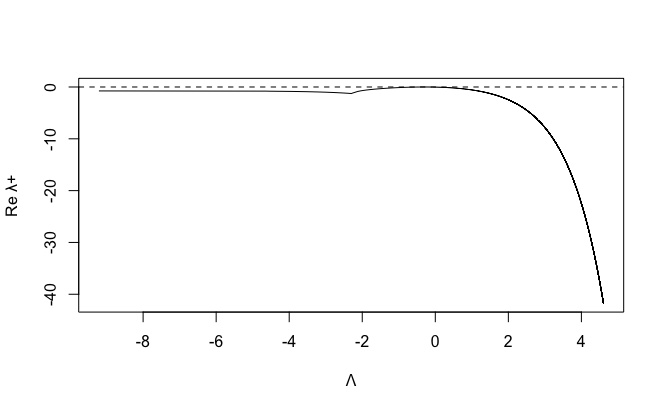
\includegraphics[width=\linewidth]{Graphs/Model2_growth-rate_vs_eigen2.png}
    \caption{\(\varepsilon=0.425\), \(\alpha_c=2\)}
  \end{subfigure}
  \caption{\textbf{Linear stability analysis.} Linear growth rates \(\lambda_\alpha\) of Laplacian modes \(\alpha=1,\ldots,N\)
  for the Schnakenberg model on a scale-free network (\(N=200\) nodes and mean degree \(\langle k\rangle=10\)) are plotted as functions of the Laplacian eigenvalues \(\Lambda_\alpha\) for the critical ratio of diffusion constants \(\sigma=22.42\). The two curves correspond to \(\varepsilon=0.425\) and \(\varepsilon=0.060\).}
  \label{fig:sch_critical_find}
\end{figure}

\begin{figure}[H] % or [htbp]
  \centering
  \begin{subfigure}{0.43\textwidth}
    \centering
    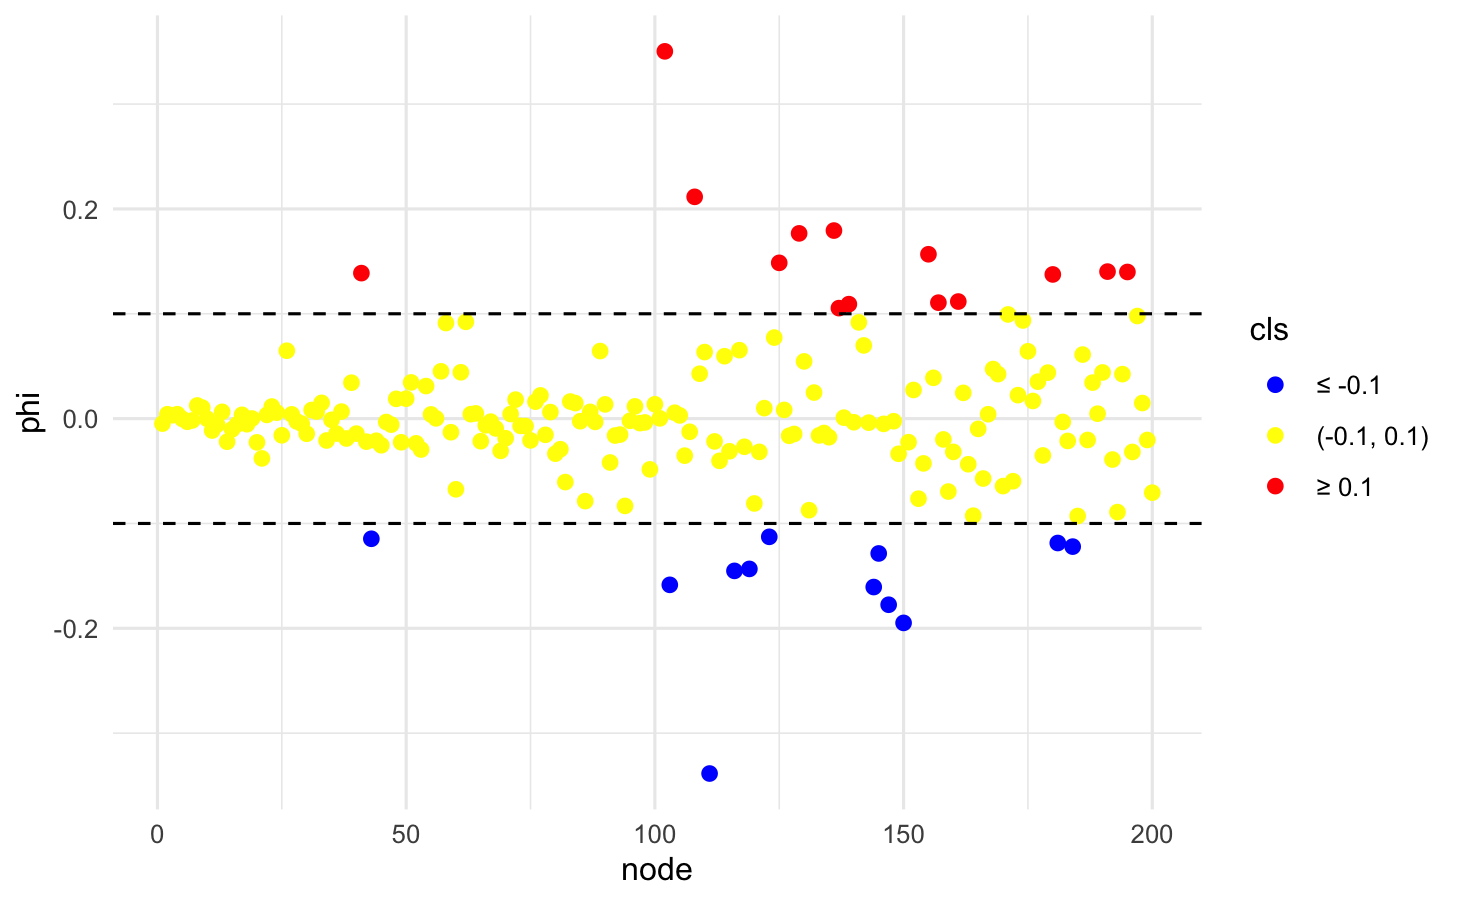
\includegraphics[width=\linewidth]{Graphs/Model2_phi66_vs_node_N=200.png}
    \caption{\(\alpha_c=66\)}
  \end{subfigure}\hfill
  \begin{subfigure}{0.43\textwidth}
    \centering
    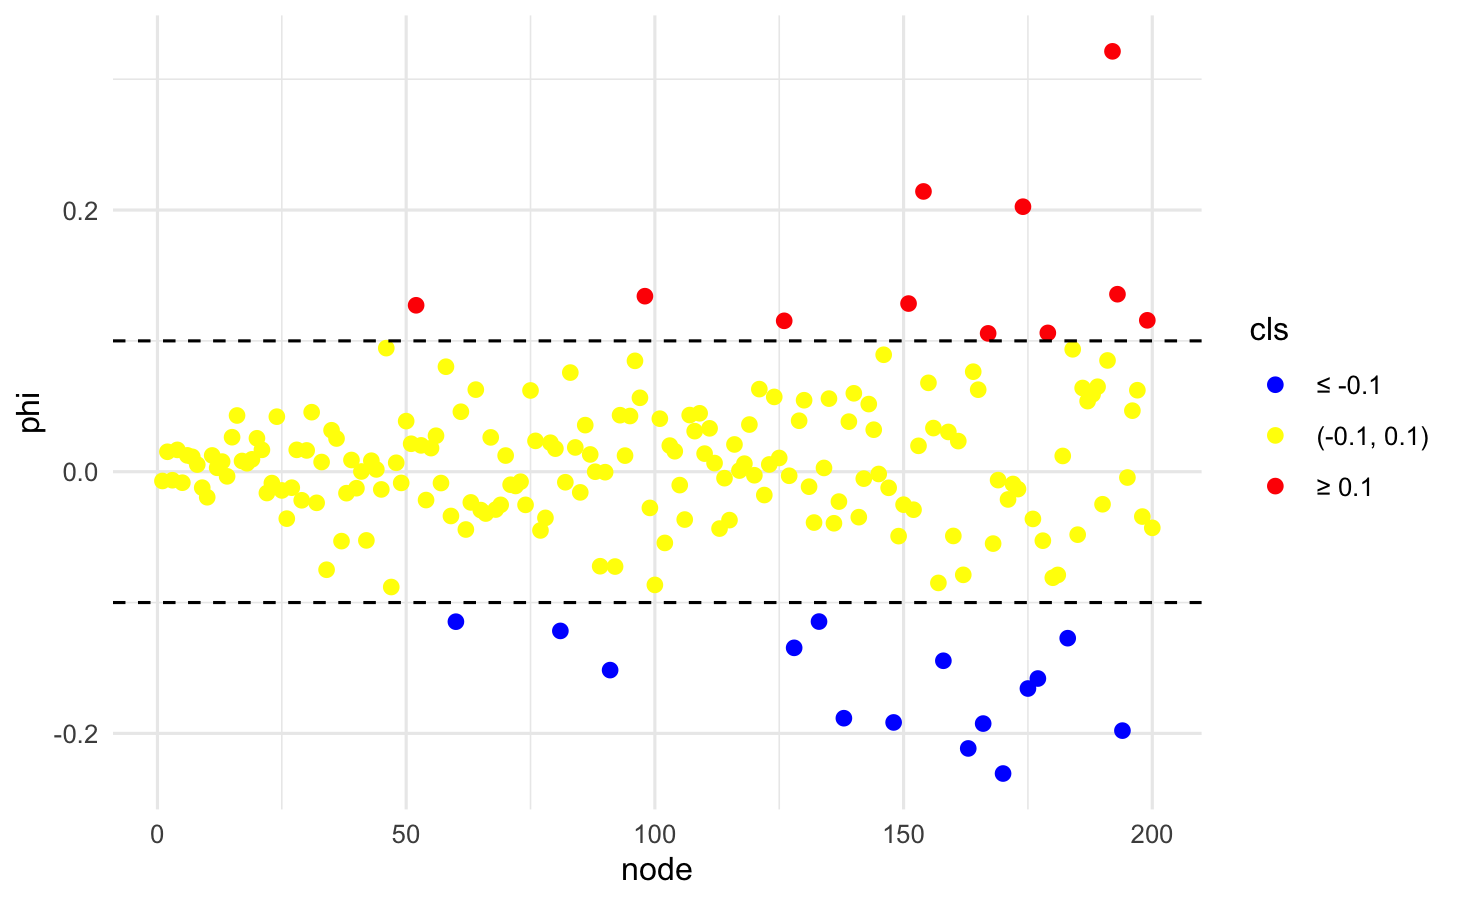
\includegraphics[width=\linewidth]{Graphs/Model2_phi2_vs_node.png}
    \caption{\(\alpha_c=2\)}
  \end{subfigure}

  \vspace{0.6em}

  \begin{subfigure}{0.33\textwidth}
    \centering
    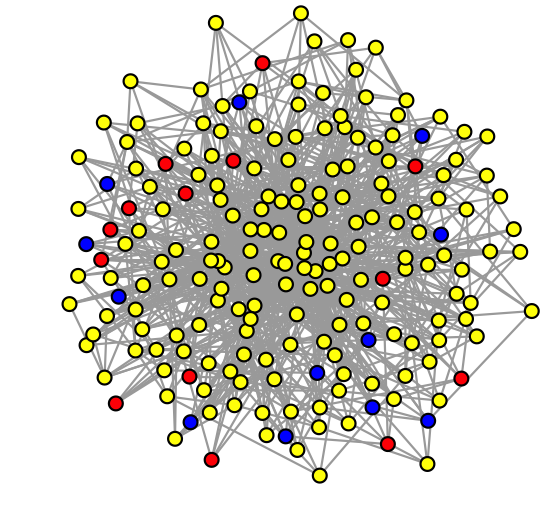
\includegraphics[width=\linewidth]{Graphs/Model2_phi66_network.png}
    \caption{\(\alpha_c=66\)}
  \end{subfigure}\hfill
  \begin{subfigure}{0.33\textwidth}
    \centering
    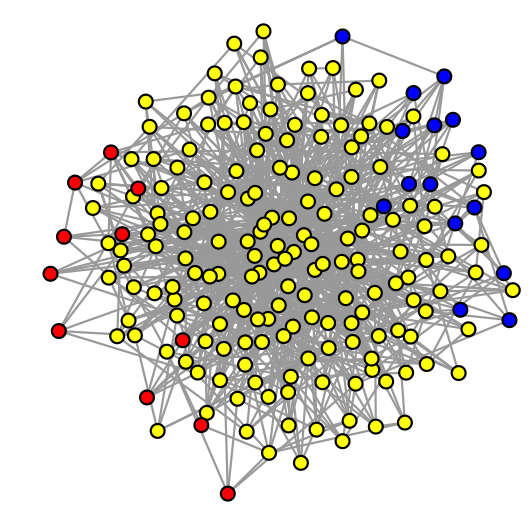
\includegraphics[width=\linewidth]{Graphs/Model2_phi2_network.png}
    \caption{\(\alpha_c=2\)}
  \end{subfigure}

  \caption{\textbf{Critical Turing modes of a scale-free network.}}
  \label{fig:sch_critical}
\end{figure}

\begin{figure}[H] % or [htbp]
  \centering
  \begin{subfigure}{0.48\textwidth}
    \centering
    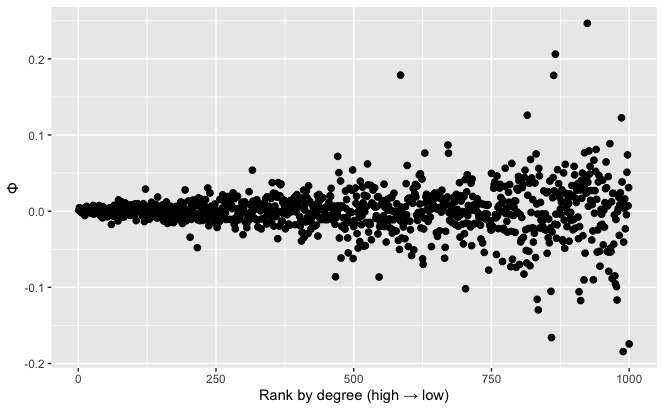
\includegraphics[width=\linewidth]{Graphs/Model2_phi_vs_index.png}
    \caption{}
  \end{subfigure}\hfill
  \begin{subfigure}{0.48\textwidth}
    \centering
    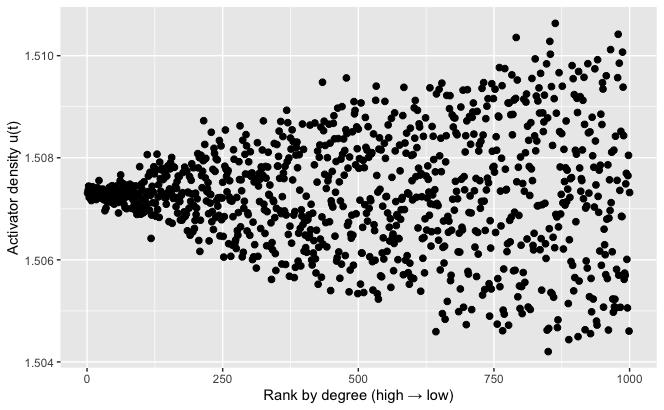
\includegraphics[width=\linewidth]{Graphs/Model2_density_vs_index_t=200.png}
    \caption{}
  \end{subfigure}

  \vspace{0.6em}

  \begin{subfigure}{0.48\textwidth}
    \centering
    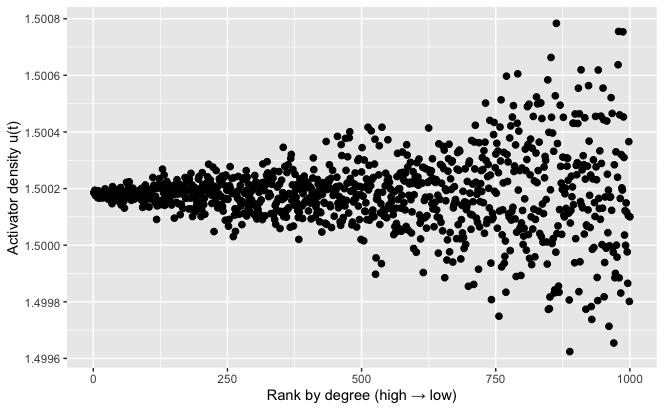
\includegraphics[width=\linewidth]{Graphs/Model2_density_vs_index_t=1000.png}
    \caption{}
  \end{subfigure}\hfill
 
  \caption{\textbf{Evolution and a Turing pattern.} The Schnakenberg model with parameters \(\varepsilon=0.12\) and \(\sigma=15.6\) on a scale-free
network of size \(N=1{,}000\) and mean degree \(\langle k\rangle=20\). Nodes are ordered according to their degrees. \textbf{a,} The critical mode (the Laplacian eigenvector with
\(\alpha_c = 2\)). \textbf{b,} The activator pattern at the early evolution stage (\(t=200\)). \textbf{c,} The stationary activator pattern at the late stage (\(t=10{,}000\)).}
\label{fig:sch_evolution}
\end{figure}

Figure~\ref{fig:sch_evolution} shows that, in the early stages, the activator densities are similar to the critical eigenvector, but as time passes, all nodes stabilize.

\section{Use of ChatGPT}

ChatGPT (OpenAI) assisted with code development, the conversion of analyses from an R Notebook to a standalone R script, and copy-editing for grammar and clarity in the final manuscript.